\documentclass[dvipdfmx]{jarticle}
\usepackage{url}
\usepackage{graphicx}
\usepackage[top=30truemm,bottom=30truemm,left=25truemm,right=25truemm]{geometry}


\begin{document}
\begin{titlepage}
    \begin{center}
        {\huge データベース 課題1レポ―ト}
        \vspace{180pt}\\
        \begin{tabular}{rl}
            氏名 & 山久保孝亮\\
            所属 & 大阪大学基礎工学部情報科学科ソフトウェア科学コース\\
            メールアドレス & u327468b@ecs.osaka-u.ac.jp\\
            学籍番号 & 09B22084\\
            提出日 & \today\\
        \end{tabular}
    \end{center}
\end{titlepage}
\section{課題1}
\subsection{SQL文}
課題1の問い合わせに答えるためのSQL文は以下のとおりである.\\\\
SELECT course.code, AVG(registration.grade)\\
    FROM course, registration\\
    WHERE course.code = registration.code AND course.credit >= 3\\
    GROUP BY course.code;
\subsection{解法}
今回の課題で使用する列は科目番号,単位数,平均点を求めるための成績の三つである.科目番号と単位数はテーブルcourse,成績はテーブルregistrationに存在する.
courseとregistrationを結合するために共通の列であるcodeを=でつないでいる.また,単位数が3以上のためcourse.credit>=3としている.
また,codeについてグループ表をまとめるのでGROUP BY course.codeとした.出力するのは科目番号であるcourse.codeと,AVG()を使って平均を計算したAVG(registration.grade)である.

\subsection{問い合わせの結果}
問い合わせの結果は以下の図1のようになる.
\begin{figure}[h]
    \centering
    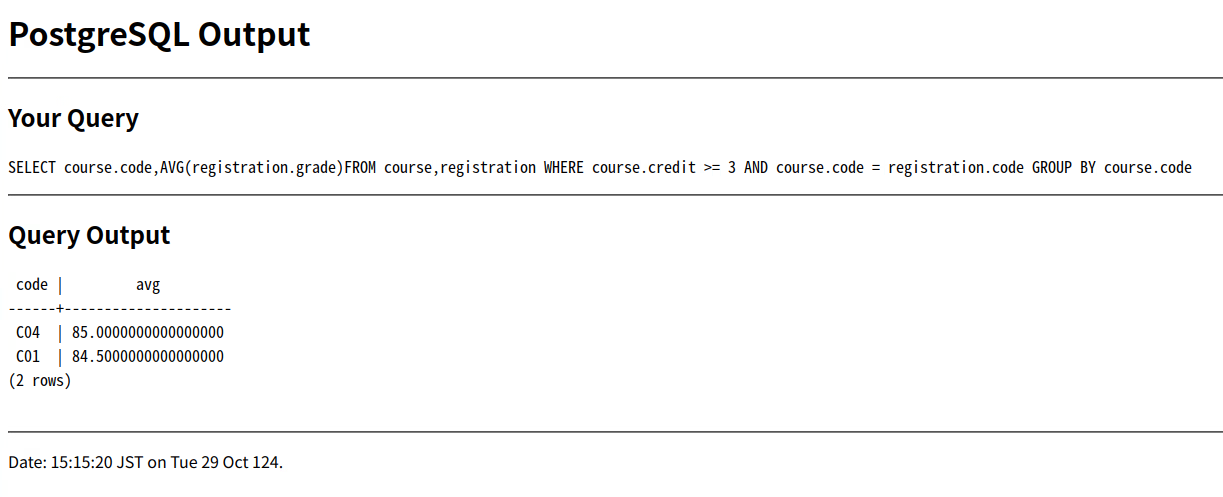
\includegraphics[width=12cm]{kadai1.png}
    \caption{課題1の問い合わせ結果}
\end{figure}
\section{課題2}
\subsection{SQL文}
課題2の問い合わせに答えるためのSQL文は以下のとおりである.
\\\\
SELECT course.code,AVG(registration.grade)\\
FROM course,registration,student\\
WHERE course.code = registration.code AND registration.number = student.number AND student.year = 2\\
GROUP BY course.code;
\subsection{解法}
今回の課題で使用する列は科目番号,学年,平均を求めるための成績の三つである.科目番号はテーブルcourse,学年はテーブルstudent,成績はテーブルregistrationに存在する.
courseにregistrationを結合するために共通の列であるcodeを,studentを結合するために共通の列であるnumberを=でつないでいる.学年が2の時のため,student.year = 2とした.
また,codeについてグループ表をまとめるのでGROUP BY course.codeとした.出力するのはcourse.codeと,AVG()を使って平均を算出したAVG(registration.grade)である.
\subsection{問い合わせの結果}
問い合わせの結果は以下の図2のようになる.
\begin{figure}[h]
    \centering
    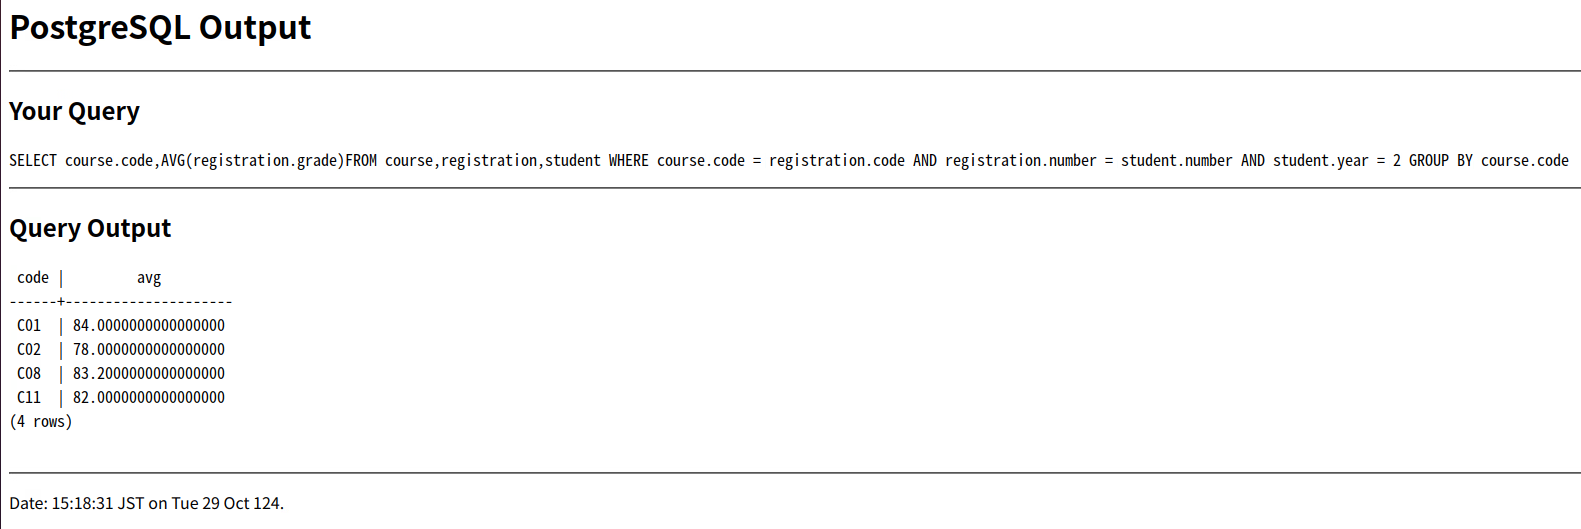
\includegraphics[width=12cm]{kadai2.png}
    \caption{課題2の問い合わせ結果}
\end{figure}
\section{課題3}
\subsection{SQL文}
課題3の問い合わせに答えるためのSQL文は以下のとおりである.
\\\\
SELECT course.code,AVG(registration.grade)\\
FROM course,registration,lecturer,lectured\_by\\
WHERE course.code = lectured\_by.code AND lectured\_by.number = lecturer.number AND lecturer.affiliation = 'ICS'\\
GROUP BY course.code; 
\subsection{解法}
今回の課題で使用する列は科目番号,平均を求めるための成績,教員の学科の三つである.
科目番号はテーブルcourse,成績はテーブルregistration,教員の学科はテーブルlecturerに存在する.
courseとlecturerには共通の列が存在しないので,まずcourseにlectured\_byを結合するために共通の列であるcodeをイコールで結ぶ.これにより,courseにnumberが追加されるので,lecturerを結合する.そしてregistrationを結合するために共通の列であるcodeを=でつないでいる.
情報科学科の教員なので,lecturer.affiliation = 'ICS'とした.また,codeについてグループ表をまとめるのでGROUP BY course.codeとした.出力するのはcourse.codeと,AVG()を使って平均を算出したAVG(registration.grade)である.
\subsection{問い合わせの結果}
問い合わせの結果は以下の図3のようになる.
\begin{figure}[h]
    \centering
    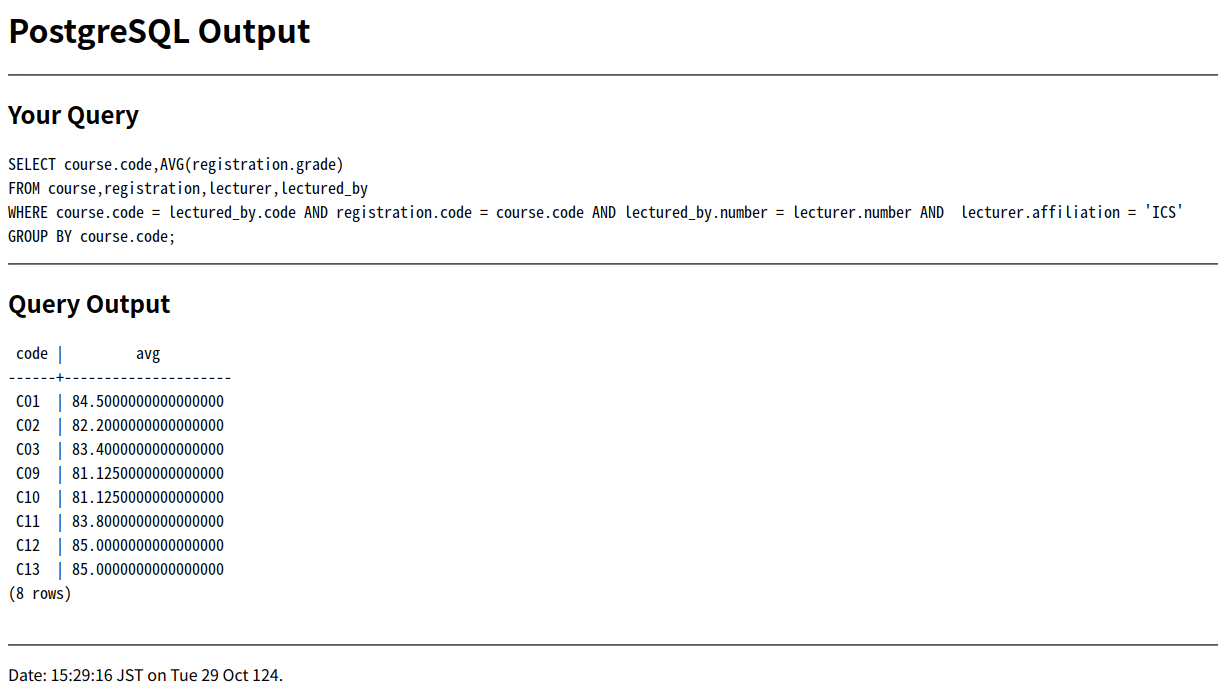
\includegraphics[width=12cm]{kadai3.png}
    \caption{課題3の問い合わせ結果}
\end{figure}
\section{課題4}
\subsection{SQL文}
課題4の問い合わせに答えるためのSQL文は以下のとおりである.
\\\\
SELECT student.name\\
FROM course,student,registration\\
WHERE course.code = registration.code AND student.number = registration.number AND course.room IS NULL;
\subsection{解法}
今回の課題で使用する列は学生名と教室の二つである.
学生名はテーブルstudent,教室はテーブルcourseに存在する.
studentとcourseには同じ列が存在しないので,どちらにも同じ列が存在するテーブルregistrationを使用して結合する.具体的には,courseにregistrationを結合するために共通の列であるcodeを,
studentを結合するために共通の列であるnumberを=でつないだ.また,教室が空値であるのでroom IS NULLとした.
\subsection{問い合わせの結果}
問い合わせの結果は以下の図4のようになる.
\begin{figure}[h]
    \centering
    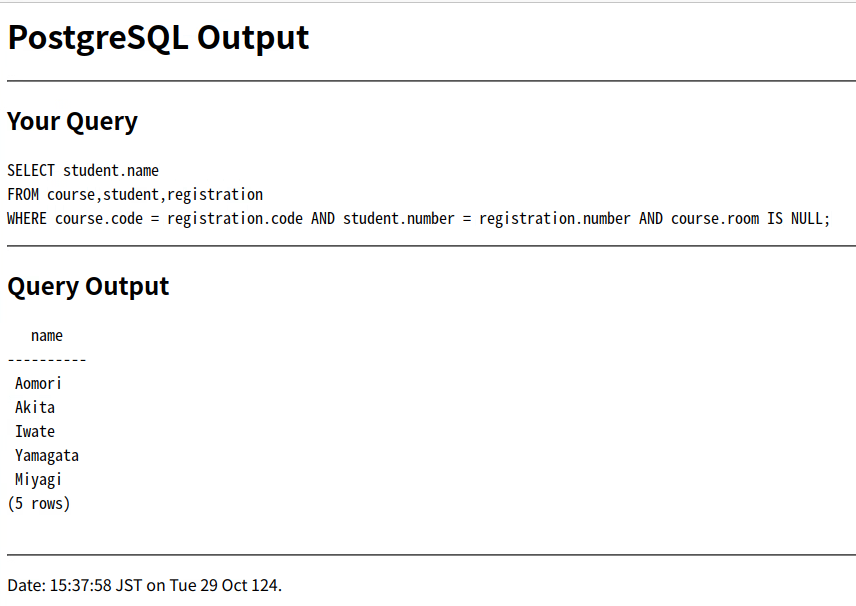
\includegraphics[width=12cm]{kadai4.png}
    \caption{課題4の問い合わせ結果}
\end{figure}
\section{感想}
今回の課題を通して私が難しいと感じたことは,必要な列を使用するためにテーブルを連結することである.特に,課題3の連結が難しく感じた.
今後の演習を見据えて教訓にしたいこととしては,それぞれのテーブルの列の内容を,色分けなどしてわかりやすく整理しておくことである.これによりどのテーブルのどの列が
共通しているのかを判断しやすくなるためである.
\end{document}